\chapter{Indledning}

\section{Baggrund}
Den demografiske udvikling er en kendt og omtalt faktor i store dele af verden og  det danske samfundet er også under pres. I Danmark bliver vi flere ældre, færre erhvervsaktive og der er et lavt fødselstal. En rapport fra KL fra 2014 beskrive alle de demografiske tendenser. Den viser, at gennemsnitsalderen er voksende. En stigende gennemsnitalder vil påvirke ældrekvoten i opadgående retning, se figur 1.1. Ældrekvoten er et udtryk for antallet af personer over 64 år pr. 100 personer i den arbejdsdygtige alder 15-64 år\cite{KL}.  Udviklingen gør, at der er færre i den arbejdsdygtige aldre til at forsørge de flere udenfor denne aldre. 

\begin{figure}[H]
\centering
\caption{Figur 1.8 fra \cite{KL}. Ældrekvoten i Danmarks kommuner fra 2004 (venstre) og fra 2014 (højre). Figuren viser, at der har været en udvikling af ældrekvoten fra 2004 til 2014, hvor største delen af Danmark har en ældrekvote over 27. Der ses, at de større byer ikke har helt så store problomer. I hovedstadsområdet er ældrekvoten under 22 i 2014. \textbf{Kilde:} Danmarks Statistik, statistikbanken, Folk1, Bef1A og BefA07. Primo året.}
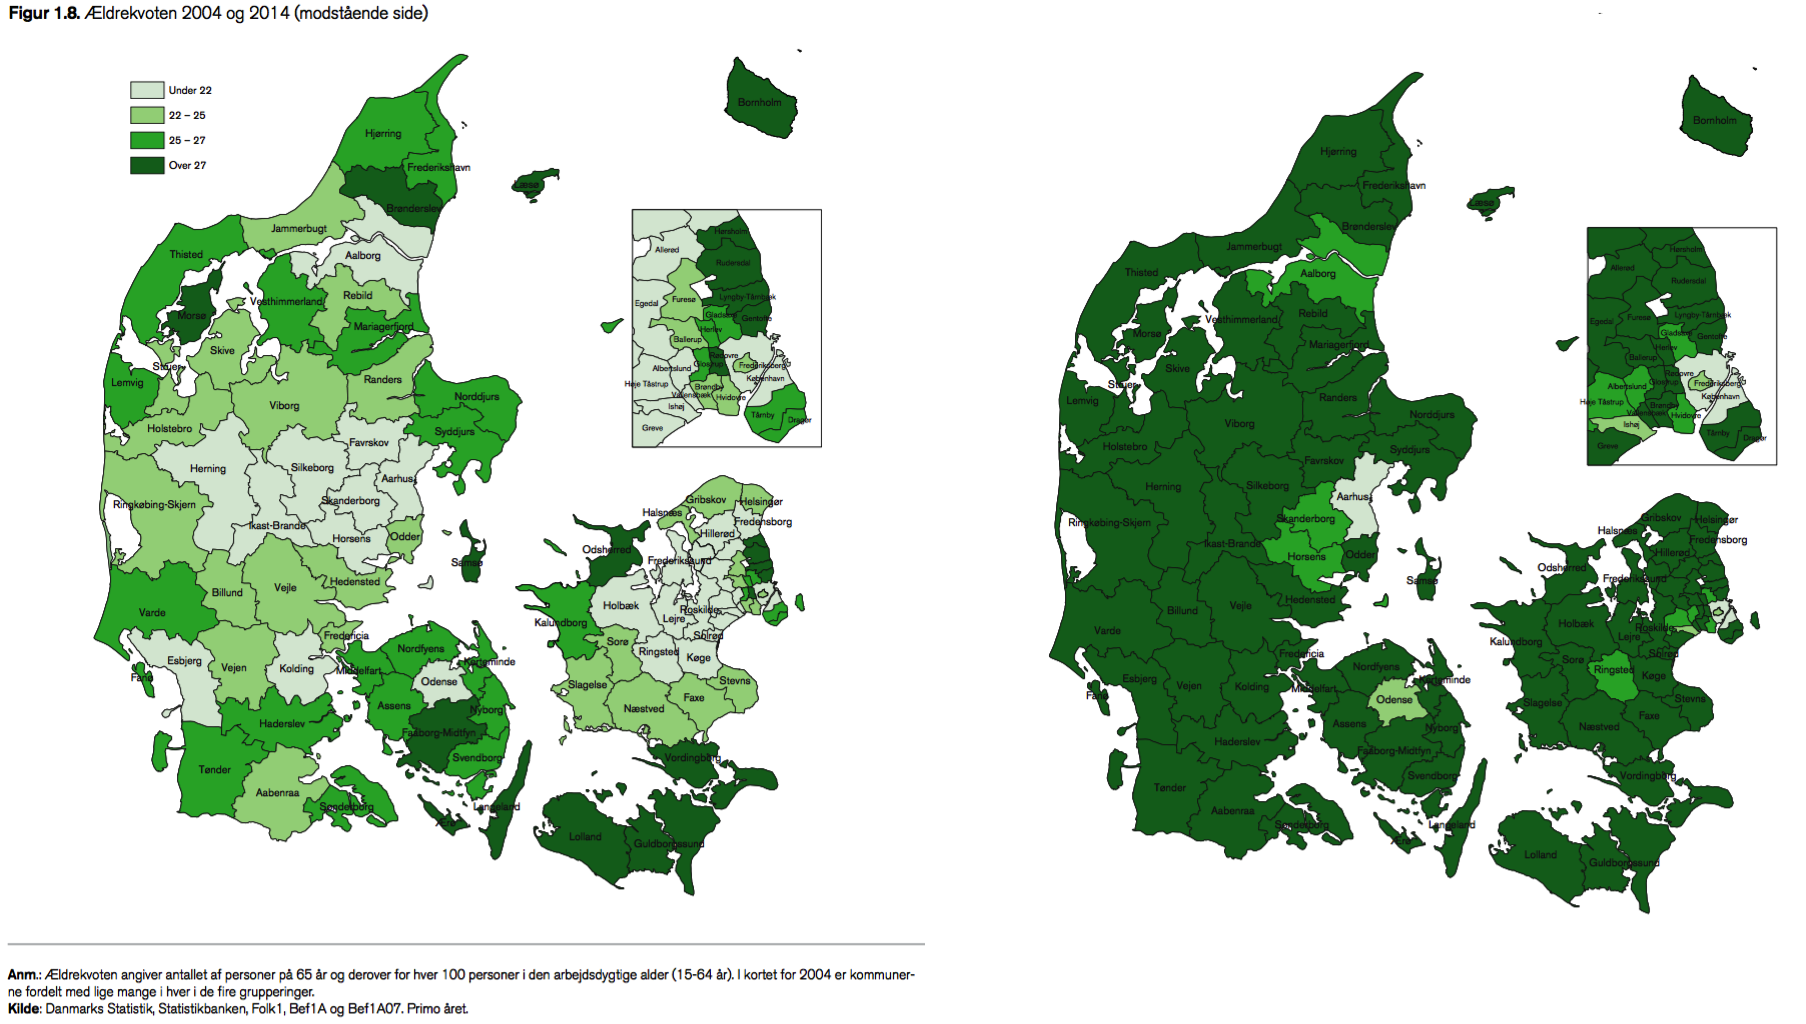
\includegraphics[width=1\textwidth]{Figurer/Snip20160428_14}
\end{figure}

Den demografiske udvikling vil på sigt skabe store problemer, særligt indenfor sundheds- og plejesektoren både samfundsøkonomisk og ressourcemæssigt. I figur 1.2 er det vist, at i år 2040 vil der for hver 100 i den arbejdsdygtige alder være 43 over plus 30 under denne aldre. Figur 1.2 klarlægger, at hvis fremskrivningen holder stik, vil der være færre og færre til at betale skat, hvilket resulterer i, at det bliver dyrere og dyrere for samfundet at forsørge de ældre. Med disse demografiske samt økonomiske udfordringer Danmark står overfor, er det nødvendigt at tænke i andre baner. Digitaliseringsstyrelsen mener, at sundhed skal leveres på nye mere smarte og teknologiske måder\cite{Digst}.

\begin{figure}[H]
	\centering
	\caption{\cite{KL} Børnekvoten og ældrekvoten, antal børn hhv. ældre pr. 100 i den erhvervsaktive alder 15-64 år. \textbf{Anm:} Tallene fra 2040 er baseret på befolkningsfremskrivninger, der bygger på gennemsnittet af en række fremskrivningsparametre over årene fra 2010-2014. \textbf{Kilde:} Danmarks Statistik, Statistikbanken, Bef1A, Folk1, Frdk113. Primo året. og Frkm113. Primå året.}
	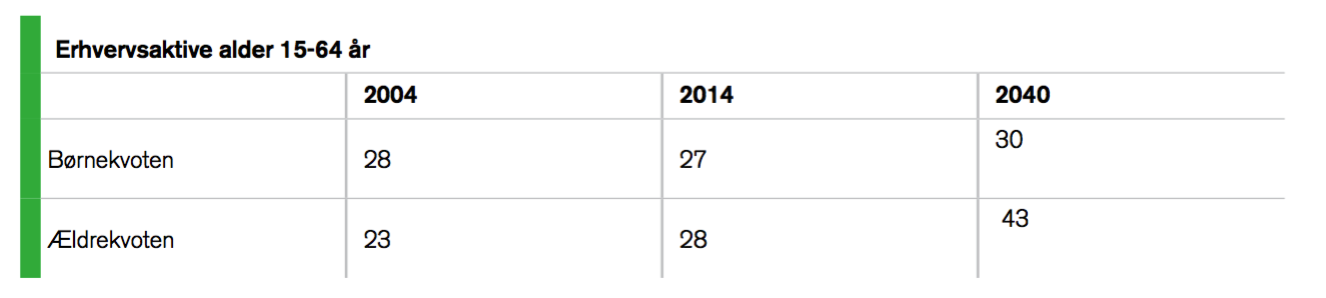
\includegraphics[width=1\textwidth]{Figurer/Snip20160513_6}
\end{figure}    

Telemedicin er derfor for alvor kommet på dagsorden hos regeringen, regionerne og kommunerne. I 2012 udarbejdede disse parter en ambitiøs national handlingsplan for udbredelsen af telemedicin i Danmark\cite{Digst}. Handleplanen skal give erfaringer med telemedicin samt mulighedden for parterne at samarbejde om at skabe fælles nationale standarder for sundheds-it med det fokus at sikre en hurtigere og mere sikker udbredelse af telemedicin til nye patientgrupper og behandlingsområder i fremtiden\cite{NationalH}.\\
Digitaliseringsstyrelsen er ved at lave en ny fællesoffentlig digitaliseringsstrategi frem mod 2020, hvor et af pejlemærkerne tager udgangspunkt i den offentlige sektor digitalisering, hvor datadeling, datasikkerhed og it-infrastruktur er temaer\cite{digst1}. Denne strategi skal understøtte de teknologiske muligheder for smartere og mere sikker deling af data mellem borger og offentlige sektor\cite{digst2}.\\
Kommunernes strategi er fokuseret bredere - nemlig på telesundhed og ikke telemedicin.

Telemedicin er en underbegreb indenfor telesundhed, hvor telesundhed indgår i det overordnede begreb velfærdsteknologi\cite{KLs}. Forholdet mellem de tre begreber er illustreret i figur 1.3. 

\begin{figure}[H]
	\centering
		\caption{Forholdet mellem velfærdsteknologi, telesundhed og telemedicin\cite{KLs}.}
	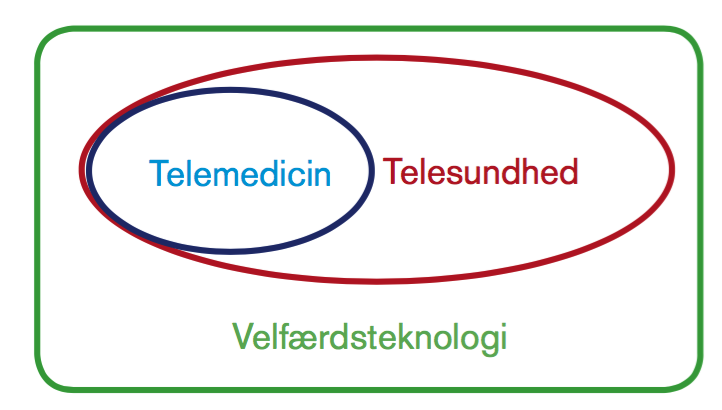
\includegraphics[width=0.6\textwidth]{Figurer/Snip20160426_6}
\end{figure}


I "Kommunernes strategi for telesundhed"\ defineres telesundhed som brugen af informations- og kommunikationsteknologi til at understøtte forebyggende, behandlende eller rehabiliterende aktiviteter over afstand. Hvorimod telemedicin mere fokuseret på selve diagnosen og behandlingen borgeren har behov for. Telesundhed fokuserer på borgernes helbred, inden de bliver patienter\cite{KLs}\cite{sundhed}.

Kommunernes mål med telesundhed er at gøre borgerne mere selvstændige, uafhængige af tid og sted og øge deres følelsen af at kunne mestre eget liv. Telesundhed skal som minimum kunne levere ydelserne af samme kvalitet som før\cite{KLs}.

Kommunerne mener, at telesundhedsløsningerne har et stort potentiale og kan være med til at varetage forskellige kommunale opgaver. I hjemmeplejen har man i flere kommuner blandt andet Viborg\cite{viborg}, Halsnæs\cite{hals} og Favrskov forsøgt sig med virtuel hjemmepleje, hvor påmindelse om medicin- og fødeindtag bliver kommunikeret over videokonference mellem borger og den sundhedsprofessionelle. 

\section{Formål}
Denne mini-MTV har til formål at vurdere virtuel hjemmepleje i Favrskov kommune. Netplan Care og Favrskov Kommune er i gang med et innovationssamarbejde om udviklingen af en kommunal digital velfærdsteknologisk sundhedsstrategi for telesundhed. 

Favrskov kommune startede op på telesundhed i 2015\cite{projektplan} på baggrund af et kørende projekt i Lyngby-Tårbæk, som havde til formål at screene KOL patienter. Lyngby-Tårbæk benyttede Appinux' telemedicinske platform og på baggrund af deres erfaringer, valgte Favrskov Appinux' løsning\cite{Karin}. De benytter nogle forskellige applikationer, men det er den virtuelle hjemmepleje via videokonferencer, denne mini-MTV vil vurdere.    

Mini-MTV'en udarbejdes i samarbejde med sundhedsteknologistuderende fra Aarhus Ingeniørhøjskole, Netplan Care og Favrskov Kommune. Analysen skal vurdere brugen af Appinux' løsning i Farvskov kommune, hvor påmindelse om medicin- og fødeindtag leveres via virtuel hjemmepleje. Den samlede vurderingen vil foreligge på baggrund af fire forskellige aspekter: teknologien, borgerne, organisation og økonomien.   

\section{Fokuserede spørgsmål}
De opstillede fokuserede spørgsmål er dem, der ønskes besvares gennem denne mini-MTV. 

\begin{itemize}
	\item Hvordan fungerer Appinux-løsningen med videokonference i Favrskov Kommune? Spørgsmålet søges besvaret med udgangspunkt i følgende punkter:
	\begin{itemize}
	\item Sikkerhedskrav
	\item Dækning %(video-conferencing, kodeks mm)
	\item Kompatibilitet 
\end{itemize}
\end{itemize}

\begin{itemize}
	\item Hvilke borgermæssige konsekvenser er der ved implementering og drift af virtuel hjemmepleje med videokonference i Favrskov Kommune? Spørgsmålet søges besvaret med udgangspunkt i følgende punkter:
	\begin{itemize}
	\item Tilfredshed
	\item Borgeraccept
	\item Trykhed
\end{itemize}
\end{itemize}

\begin{itemize}
	\item Hvilke organisatoriske konsekvenser er der ved implementering og drift af virtuel hjemmepleje med videokonference sammenlignet med konventionel fysisk hjemmepleje i Favrskov Kommune? Spørgsmålet søges besvaret med udgangspunkt i følgende punkter:
	\begin{itemize}
	\item Forskel i medarbejdernes arbejdsgange før/efter virtuel hjemmepleje
	\item Medarbejdernes reaktion
	\item Beslutningsgrundlag for valg af Appinux-løsningen 
\end{itemize}
\end{itemize}


\begin{itemize}
	\item Hvilke økonomiske omkostninger er der ved implementering og drift af virtuel hjemmepleje med videokonference sammenlignet med konventionel fysisk hjemmepleje i Favrskov Kommune?
\end{itemize}

